%% question-11.tex
%%

%% ==============================
\subsection{Modélisation explicite d'une action}
\label{sec:question11}
%% ==============================

Le concept d'action est présenté à l'aide de la figure \ref{fig:action}. Une \emph{Action} est parent de 6 enfants : \emph{SeDeplacer}, \emph{UtiliserItem}, \emph{Revetir}, \emph{Frapper}, \emph{Tirer} et \emph{ConsulterRadar}.

Cest un personnage qui dispose de ces \emph{Action}.

\begin{figure}
	\centering
	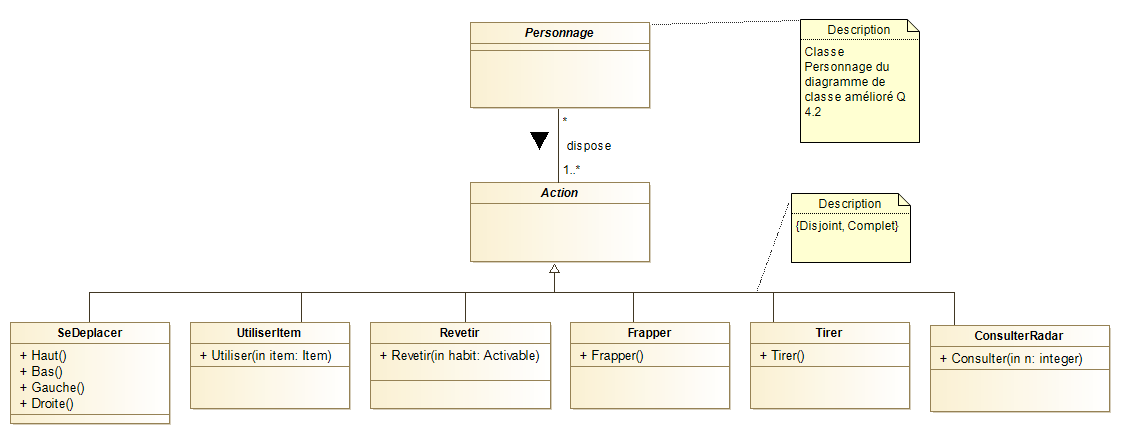
\includegraphics[width=500pt]{assets/class__Action}
	\caption{Diagramme de classe d'une action}
	\label{fig:action}
\end{figure}